\begin{frame}{Mass of \chiboneThreeP in $\chib \to \Y3S \gamma$ decay (2)}
\begin{center}
The measured $m_{\chiboneThreeP}$=\textcolor{red}{$10{,}508\pm2\stat\pm8\syst\mevcc$} is consistent
with the mass measured in another study with converted photons ---
\textcolor{blue}{$10{,}510\pm3.0\stat^{+4.4}_{-3.4}\stat\mevcc$}.
% 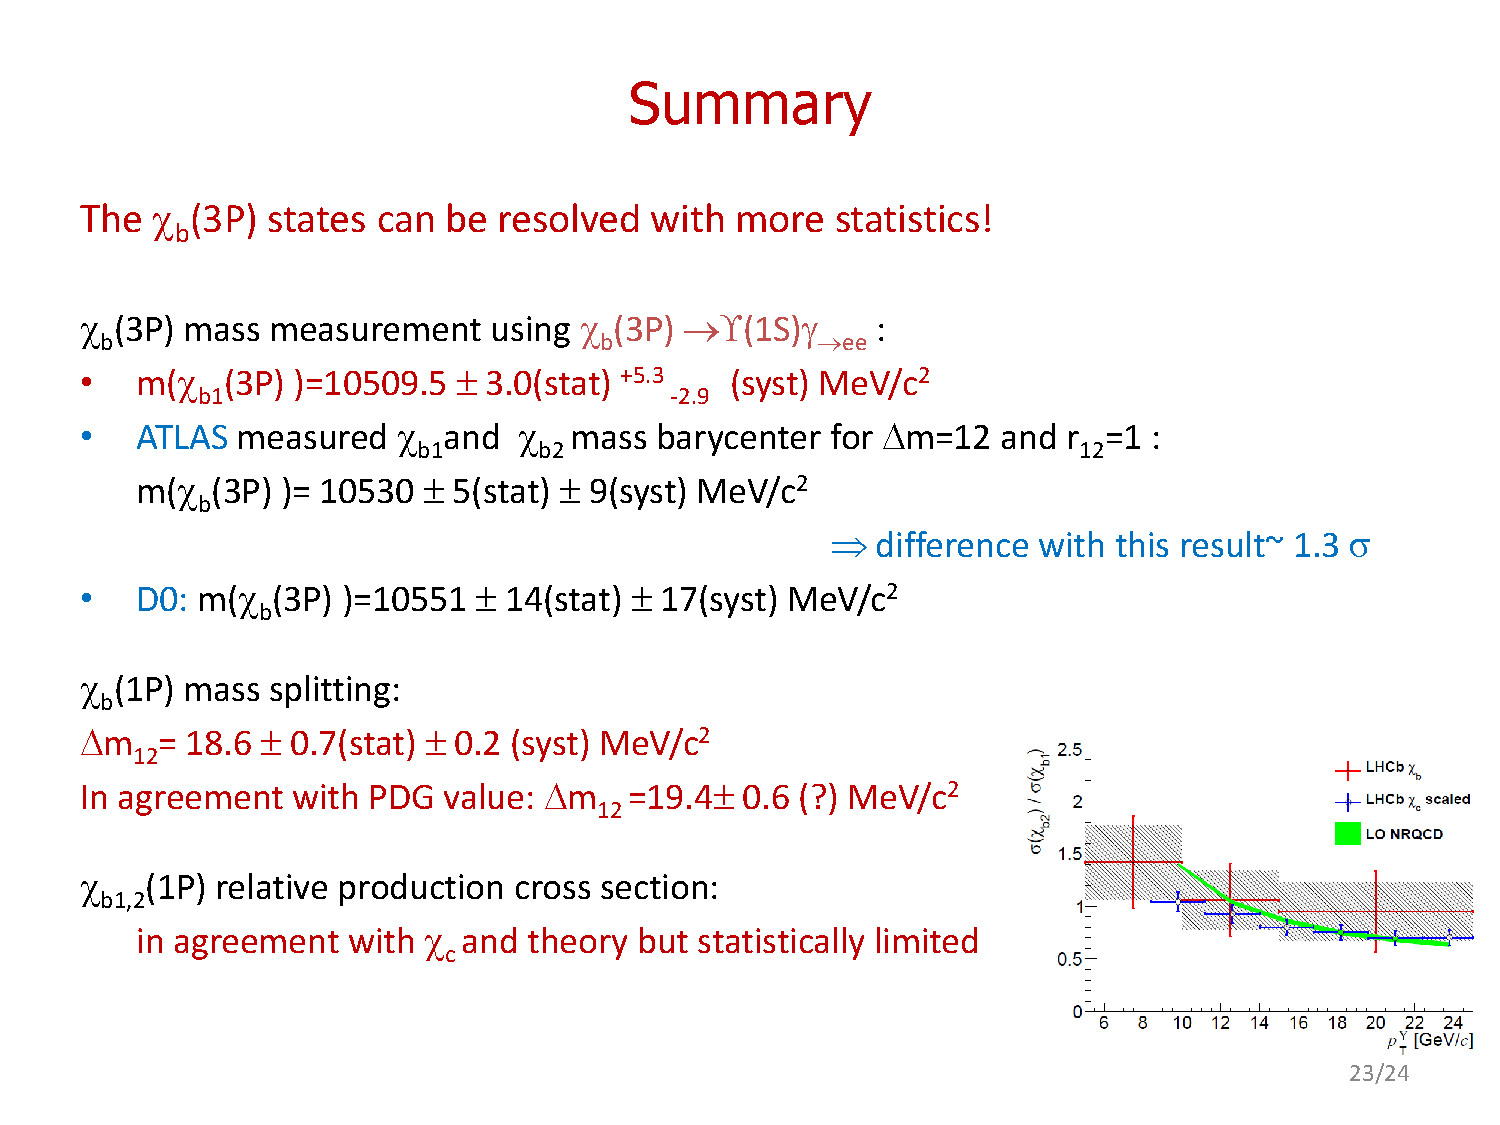
\includegraphics[width=85mm]{m3p-converted/converted}
\end{center}
\begin{itemize}
\item \atlas measured $\chi_{b1}$ and $\chi_{b2}$  mass barycenter for $m_{\chi_{b2}} - m_{\chi_{b1}}=12\mevcc$ and $\lambda=0.5$:
\textcolor{blue}{$m_{\chibThreeP} = 10{,}530\pm5\stat\pm9\syst\mevcc$}
\item D0: \textcolor{blue}{$m_{\chibThreeP} = 10{,}551\pm14\stat\pm17\syst\mevcc$}
\end{itemize}
\end{frame}
